\section{Численные эксперименты}\label{sec:experiments}

Мы сравниваем методы по числу обращений к оракулу на цепочках S и X
(трудных семействах из раздела~\ref{sec:lower-origin}),
на пуассоновских моделях и на 65 задачах из 13 семейств (по пять
экземпляров каждого), включая суммы квартических функций и логистическую
регрессию. Число запросов делится на $n$, то есть измеряется в проходах
по данным; учитываются и запросы, потраченные на неудачные пробные точки
при подборе шага.
Относительная невязка равна $(f-f_{\rm ref})/\widehat\Delta$,
где $\widehat\Delta=f(0)-f_{\rm ref}$, а $f_{\rm ref}$ --- эталонное
значение минимума. На цепочках оно совпадает с $f^\ast$, известным
из построения. На остальных задачах $f^\ast$ неизвестно, и $f_{\rm ref}$ ---
его приближение, найденное численно заранее; поэтому мы обозначаем его
$f_{\rm ref}$, а не $f^\ast$. Запросы, потраченные на вычисление эталона,
в сравнении не учитываются.
Постановки задач, настройки методов и подробные результаты приведены
в приложении~\ref{app:experiments}.

\begin{figure}[p]
 \centering
 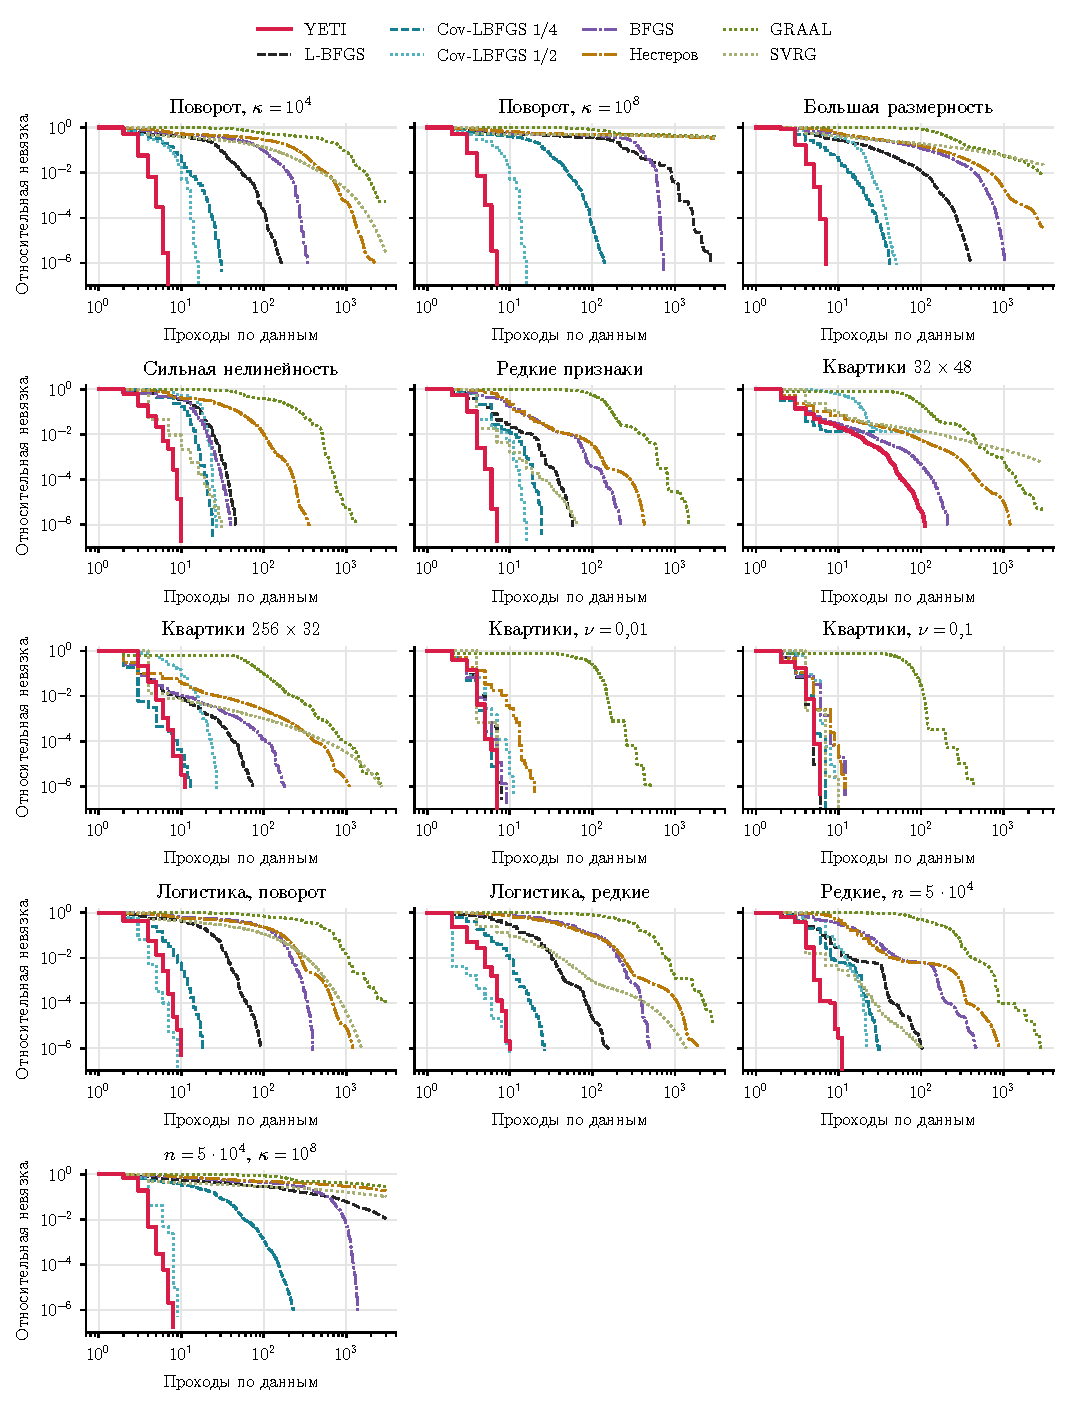
\includegraphics[width=\linewidth]{figures/families.pdf}
 \caption{Наименьшая достигнутая к данному моменту относительная невязка на первом экземпляре
 каждого семейства (обе шкалы логарифмические; YETI выделен красным; $\kappa$ --- число
 обусловленности ковариационной матрицы признаков).}
 \label{fig:exp-families}
\end{figure}

На цепочках YETI работает примерно так же, как L-BFGS. На пяти
пуассоновских задачах он достигает относительной точности $10^{-4}$
за 4--9 проходов; на freMTPL2freq методу SAGA требуется меньше проходов:
5 против 7 (табл.~\ref{tab:exp-chains}, \ref{tab:exp-glm}).

\paragraph{Остановка.}\label{sec:exp-certificate}
Критерий остановки по истории запросов~\eqref{eq:history-stop} не использует
эталонное значение. При $\varepsilon=10^{-6}\widehat\Delta$ он срабатывает
на всех 65 задачах, и все возвращённые точки удовлетворяют допуску
относительно эталона. Медиана числа проходов до остановки равна 15,
максимум --- 273. Критерий может срабатывать позже, чем допуск фактически
достигнут (рис.~\ref{fig:exp-certificate}).

\paragraph{Тестовые задачи.}
Цепочки S и X --- численные варианты трудных семейств из
раздела~\ref{sec:lower-origin}. Пуассоновские модели --- это синтетические задачи
и задачи на данных Bike Sharing и freMTPL2freq. Тринадцать семейств,
из которых составлены 65 задач (их названия указаны на рис.~\ref{fig:exp-families}
и в табл.~\ref{tab:exp-series}), устроены следующим образом.
\begin{itemize}
\item \emph{Поворот, $\kappa$}: пуассоновская регрессия, в которой
ковариационная матрица признаков имеет число обусловленности
$\kappa\in\{10^4,10^8\}$ и не диагональна в исходном базисе (её собственные
векторы повёрнуты относительно координатных осей).
\item \emph{Большая размерность}: пуассоновская регрессия с большим числом
признаков: $n=600$, $d=160$, $\kappa=10^4$.
\item \emph{Сильная нелинейность}: пуассоновская регрессия, в которой
истинный вектор параметров, по которому генерируются отклики, в три раза
длиннее, чем в остальных пуассоновских семействах; это увеличивает разброс
линейных предикторов $a_i^{\mathsf T}x$ и значений экспоненты.
\item \emph{Редкие признаки} и \emph{Редкие, $n=5\cdot10^4$}: пуассоновская
регрессия с разреженными признаками; во втором семействе число слагаемых
равно $5\cdot10^4$.
\item \emph{$n=5\cdot10^4$, $\kappa=10^8$}: плохо обусловленная
пуассоновская регрессия с $5\cdot10^4$ слагаемыми.
\item \emph{Квартики}: суммы квартических функций
$f_i(x)=\frac12(x-c_i)^{\mathsf T}H_i(x-c_i)+\frac\nu4\norm{x-c_i}^4$,
где $H_i\succ0$, а $c_i$ --- случайные центры. В названиях семейств
$32\times48$ и $256\times32$ указаны число слагаемых $n$ и размерность $d$;
$\nu$ --- вес слагаемого четвёртой степени (в этих двух семействах
$\nu=10^{-6}$).
\item \emph{Логистика, поворот} и \emph{Логистика, редкие}: регуляризованная
логистическая регрессия с повёрнутыми и с разреженными признаками
соответственно.
\end{itemize}
\FloatBarrier
